% Hallucination and Citation Verifier for Policy Question Answering
% IEEE conference format (IEEEtran). Version 2 of the paper, 20 November 2026:
% updated to the final system (git tag v2-final-test) and its final evaluation.
% Compile with pdfLaTeX (e.g. on Overleaf). Needs: fig_table_row_check.png in the same folder.

\documentclass[conference]{IEEEtran}
\IEEEoverridecommandlockouts

\usepackage{cite}
\usepackage{amsmath,amssymb,amsfonts}
\usepackage{graphicx}
\usepackage{textcomp}
\usepackage{xcolor}
\usepackage{booktabs}
\usepackage{array}
\usepackage{url}
\usepackage{tikz}
\usetikzlibrary{positioning,arrows.meta,shapes.geometric,fit,calc}
\usepackage{pgfplots}
\pgfplotsset{compat=1.17}

\newcommand{\SUP}{\textsc{Sup}}
\newcommand{\REF}{\textsc{Ref}}
\newcommand{\NEU}{\textsc{Neu}}
\newcommand{\code}[1]{\texttt{#1}}
% A new centred author row (standard IEEEtran workaround).
\makeatletter
\newcommand{\linebreakand}{\end{@IEEEauthorhalign}\hfill\mbox{}\par\mbox{}\hfill\begin{@IEEEauthorhalign}}
\makeatother

\begin{document}

\title{Hallucination and Citation Verifier\\for Policy Question Answering}

\author{
\IEEEauthorblockN{Diya Nambiar}
\IEEEauthorblockA{\textit{Department of Computing Technologies}\\
\textit{(CTECH)}\\
\textit{SRM Institute of Science and Technology}\\
Kattankulathur, Tamil Nadu, India\\
RA2411003010959}
\and
\IEEEauthorblockN{Abhishek Verma}
\IEEEauthorblockA{\textit{Department of Computing Technologies}\\
\textit{(CTECH)}\\
\textit{SRM Institute of Science and Technology}\\
Kattankulathur, Tamil Nadu, India\\
RA2411003012011}
\and
\IEEEauthorblockN{Tusharika Suman}
\IEEEauthorblockA{\textit{Department of Computing Technologies}\\
\textit{(CTECH)}\\
\textit{SRM Institute of Science and Technology}\\
Kattankulathur, Tamil Nadu, India\\
RA2411003010650}
\linebreakand
\IEEEauthorblockA{Under the guidance of Dr. P. Akilandeswari}
}

\maketitle

\begin{abstract}
Questions about attendance, examinations, hostels or scholarships look like retrieval problems, but one
wrong figure, a value read from the wrong table row, or a citation that does not say what it is credited
with can mislead a student who cannot easily check. This paper presents a fully local assistant for
institutional policy documents that treats an answer as a set of atomic claims. A local language model
(Qwen3.5 9B via Ollama) writes schema-constrained claims with section citations over hybrid BM25 and
dense retrieval. Each claim passes citation resolution, a DeBERTa-v3 NLI verifier on sentence- and
table-row-level evidence units, a numeric guard and a deterministic table-row check; a relevance gate and
an abstention rule then decide what is shown. We report an ingestion audit that found table data deleted
by a header filter, repair it, and add a seventh document. On a final test of 99 questions written
independently of the system and run once, the system declined 15 of 16 unanswerable questions and, read by
hand, presented no false statement as verified (0/99, 95\% CI 0--3.7\%); the automatic hallucination count
was 3.0\% against 9.1\% without verification. The price is coverage: 25 of 83 answerable questions were
declined, so accuracy was 62.6\% [52.8--71.5] against 79.8\% with verification off. In 17 of those 25
questions the declined claims had been verified as true and were rejected by the relevance gate, which was
tuned for a smaller model. An earlier version, evaluated on 71 other held-out questions, reached 76.1\%
accuracy with 1.4\% hallucination. The test sets are small and cover one institution.
\end{abstract}

\begin{IEEEkeywords}
hallucination detection, citation verification, retrieval-augmented generation, natural language
inference, selective answering, abstention, table question answering, policy question answering
\end{IEEEkeywords}

% ===========================================================================
\section{Introduction}
% ===========================================================================
Students ask policy questions in everyday language: how much attendance is needed to sit an exam, what
attendance code a 90\% record receives, whether a parent may stay in the hostel. The answers sit in long
documents full of tables, numbered clauses and exceptions. A general-purpose language model answers
fluently whether or not the documents support it. In this domain the damaging errors are specific: an
invented amount, a threshold borrowed from a neighbouring table row, a rule stated without its exception,
or a confident answer to a question the policy never addresses.

Retrieval-augmented generation (RAG) \cite{lewis2020rag} reduces reliance on parametric memory but does
not guarantee that generated text is entailed by the retrieved passages; unfaithful content is a
documented problem in generation generally \cite{maynez2020faithfulness}. Self-revision by the generator is
not a dependable remedy in the setting studied in \cite{huang2024selfcorrect}. A practical assistant
therefore needs a check that is independent of the generator, and a defined way of saying that the policy
does not answer.

We describe and evaluate such an assistant. The language model returns a list of atomic claims, each
tagged with the policy sections it relies on. Each claim is verified on its own, so one unsupported claim
can be removed without discarding the answer, and a refuted claim can be shown beside the policy sentence
that contradicts it. The contributions are:
\begin{enumerate}
\item A claim-level pipeline combining citation resolution, sentence- and row-level NLI, a deterministic
numeric guard, a deterministic \emph{table-row check} that resolves range look-ups the NLI model cannot,
a relevance gate and abstention, using only local models (Section~\ref{sec:system}).
\item A structure-preserving ingestion for PDF and HTML policies, motivated by an audit showing that a
common header/footer heuristic had silently deleted table values and corrupted an evaluation label.
\item A final evaluation on 99 questions from three independently written sets, converted to the scoring
format before the system was run and run once, with 95\% Wilson intervals, a verification on/off
comparison and a manual reading of every case the scorer counts as a hallucination.
\item A tuning-split analysis of four retrieval add-ons, and an error analysis that locates most remaining
errors in the relevance gate rather than in the verifier.
\end{enumerate}
The claims are deliberately limited: the sets are small, the corpus is seven documents of one
institution, and there is no external baseline.

% ===========================================================================
\section{Technical Background and Related Work}
% ===========================================================================
\subsection{Faithfulness, entailment and quantities}
Maynez et al. \cite{maynez2020faithfulness} distinguished intrinsic hallucinations (distortions of the
source) from extrinsic ones (content absent from the source) and found that entailment-based measures agree
with human judgments better than overlap metrics. We adopt the entailment view but apply it to individual
claims. ContractNLI \cite{koreeda2021contractnli} frames verification over long documents as
document-level NLI with entailed, contradicted and not-mentioned labels and evidence spans; these map to
the \SUP, \REF\ and \NEU\ verdicts of our verifier and to our requirement that every claim cite a section.
EQUATE \cite{ravichander2019equate} showed that NLI models handle quantitative reasoning weakly. Policy
tables are full of such constructs (``rank 7,001--9,000 receives 25\%''), which motivates both a numeric
guard and the table-row check introduced here.

\subsection{Abstention, self-checking and testing}
Kamath et al. \cite{kamath2020selective} formalised selective question answering, where a model may decline
and is judged by accuracy at a given coverage. We take from it the view that declining has its own
correctness criterion, so we report correct and false abstention separately. Huang et al.
\cite{huang2024selfcorrect} found that models asked to revise their own reasoning without external feedback
do not improve; we therefore verify with a separately trained model that shares no weights with the
generator. CheckList \cite{ribeiro2020checklist} proposed behavioural testing by capability; our question
categories (numeric, unanswerable, false premise, negation/exception, cross-policy) follow that spirit.

\subsection{Retrieval and verification components}
BM25 \cite{robertson2009bm25} and dense retrieval capture different signals, and Reciprocal Rank Fusion
(RRF) \cite{cormack2009rrf} merges their rankings. The dense encoder is BGE \cite{xiao2023cpack,bge}.
SummaC \cite{laban2022summac} showed that sentence-level NLI with aggregation makes NLI-based consistency
checking effective; our evidence units follow this idea. The verifier is a DeBERTa-v3
\cite{he2021debertav3} NLI checkpoint \cite{laurer}. Calibration uses expected calibration error and
temperature scaling \cite{guo2017calibration}. A dedicated fact-checker such as MiniCheck
\cite{tang2024minicheck} is a natural baseline but was not evaluated.

\subsection{Research gap}
These works address pieces of the problem. A small institutional deployment lacks an end-to-end, locally
runnable system that (i)~verifies at claim level against the \emph{cited} section, (ii)~separates whether a
citation exists from whether it supports the claim, (iii)~reads the table-structured content where policy
answers often live without losing row structure, (iv)~abstains, and (v)~is evaluated on questions written
by someone other than the builder. This paper addresses that gap at small scale and reports where it falls
short.

% ===========================================================================
\section{Problem Formulation and System Architecture}\label{sec:system}
% ===========================================================================
\subsection{Formulation}
Let $\mathcal{D}$ be a corpus of policy sections and $q$ a question. A generator, conditioned on retrieved
passages, returns claims $\{(c_i,S_i)\}_{i=1}^{n}$, where $S_i$ is the set of cited section identifiers. A
verifier assigns each claim a verdict $v_i\in\{\SUP,\REF,\NEU\}$ and a score $s_i\in[0,1]$; a relevance
gate assigns $\mathrm{rel}_i\in\{\text{on topic},\text{off topic},\text{unjudged}\}$. The kept set is
\begin{equation}
K=\{\,i:\; v_i=\SUP,\; s_i\ge\tau_s,\; \mathrm{rel}_i\neq\text{off topic}\,\},\label{eq:kept}
\end{equation}
with $\tau_s=0.5$. The assistant answers when $|K|\ge m$ ($m=1$) and otherwise declines; it also declines
when no passage is retrieved or no claim is produced. The design is deliberately asymmetric: wrongly
standing behind a claim shows a student a false statement with a citation attached, whereas wrongly
withholding a true one is visible and recoverable.

\subsection{Pipeline}
Figs.~\ref{fig:arch} and \ref{fig:claim} show the architecture and the path of one claim; the decision
logic below is taken from the implementation.

\textit{Ingestion.} PDF and HTML policies are parsed into sections. Every table row is written as one
self-describing line (``Attendance rounded to: 85 to 94\% $|$ Code: 9.''). In PDFs, tables are located with
a table finder \cite{pymupdf}; a position covered by a merged cell is filled with the text of the cell whose
bounding box contains it (a cell can be merged downwards or sideways, so copying from the row above is
wrong); a table continued on the next page inherits its header; contents tables are dropped; page text is
read top to bottom. Running headers and footers are removed only when they occur within the first or last
three text lines of at least three pages. In HTML, merged cells are expanded from their \code{rowspan} and
\code{colspan}. Headings are detected from numbered, Roman-numeral, regulation-style (``R~7.1'') and
all-capitals lines.

\textit{Audit finding.} The previous heuristic removed \emph{any} short line repeated three or more times in
a PDF. Because a table cell is often its own line, it deleted 628 lines of the academic regulations,
including every grade point, two attendance codes, the class/CGPA bands and every ``\%'' sign. One held-out
evaluation label had been written from this damaged text and was corrected (Section~\ref{sec:disclosure}).

\textit{Retrieval.} Embeddings (BGE-base-en-v1.5, 768-d) are held in ChromaDB and a BM25 index in memory.
Dense and BM25 rankings over a 50-candidate pool are fused by
\begin{equation}
\mathrm{RRF}(d)=\sum_{r\in\{\mathrm{dense},\,\mathrm{bm25}\}}\frac{1}{k+\mathrm{rank}_r(d)},\quad k=60,
\end{equation}
keeping the top 6 passages with at most two chunks per section; chunks are at most 1800 characters.

\textit{Generation.} Qwen3.5 9B \cite{qwen3,qwen35} writes the answer as JSON constrained to a claim schema
at temperature 0 with ``thinking'' disabled. The prompt asks for one fact per claim, and for a question
built on a false premise to state what the passages actually say instead of returning nothing.

\textit{Citation resolution.} A claim with no citation, or none that resolves, is \NEU\ with score 0. A
cited section must exist among the retrieved passages or in the corpus; existence alone never grants
support. A clause number cited from inside a retrieved passage is mapped back to that passage only when
exactly one passage contains it.

\textit{NLI evidence units.} Each resolved chunk is scored against the claim by a DeBERTa-v3
MNLI/FEVER/ANLI checkpoint on CPU. A verbatim quote of at least 40 normalised characters and 6 words is
entailed without the model. Otherwise sentences are scored first, then 2--3-sentence windows and list items
with their lead-in. Table rows are separate units, never joined to neighbours. For chunk $j$ with units
$U_j$, let $e_j=\max_{u\in U_j}P_{\mathrm{ent}}(c\mid u)$ and $k_j=\max_{u\in U_j}P_{\mathrm{con}}(c\mid u)$;
across all resolved chunks $\sigma=\max_j e_j$ and $\kappa=\max_j k_j$, so citation order cannot change the
verdict. Let $\kappa_p$ be the same maximum over prose units only.

\textit{Numeric guard.} Let $\mathcal{N}(c)$ be the numbers in the claim (bare 0, 1, 2 ignored) and
$\mathcal{N}(S)$ those in all resolved chunks. The guard $G$ holds when every element of $\mathcal{N}(c)$
equals some element of $\mathcal{N}(S)$; it can veto support but never grant it.

\textit{Table-row check.} NLI cannot place 90\% inside ``85 to 94\%'', reads a neighbouring row as a
contradiction, and scores ``Header: value'' rows poorly. Let $R$ be the table rows of the resolved chunks,
$W(\cdot)$ the content words (stemmed; single-letter codes kept), $M(c)$ the words the claim capitalises
mid-sentence, and $\mathcal{I}(r)$ the numeric ranges a row states (``$a$ to $b$'', ``$\ge a$'',
``below $b$'', ``top $b$''). A row $r$ \emph{matches} $c$ when
\begin{itemize}
\item every $x\in\mathcal{N}(c)$ is in $\mathcal{N}(r)$ or in some interval of $\mathcal{I}(r)$, and at least
one is in $\mathcal{N}(r)$ exactly;
\item $|W(c)\cap W(r)|/|W(c)|\ge 0.6$ and $M(c)\subseteq W(r)$;
\item no claim word belongs only to another row: $W(c)\cap\bigcup_{r'\neq r}W(r')\subseteq W(r)$;
\item each exactly matched number lies in a cell whose own header or value words intersect $W(c)$.
\end{itemize}
Let $T$ be the event that \emph{exactly one} row matches. The check can grant support but never refutes.

\textit{Verdict.} With $\tau_e=0.5$, $\tau_c=0.9$ and $\mathcal{C}$ the event that one cited section
supports the claim while a different one contradicts it in prose at $\ge\tau_c$, rules apply in order:
\begin{equation}
(v,s)=\begin{cases}
(\NEU,\sigma/2) & \sigma\ge\tau_e\wedge\mathcal{C},\\
(\SUP,0.9) & (\sigma<\tau_e\vee\neg G)\wedge T\wedge\kappa_p<\tau_c,\\
(\REF,\kappa) & \sigma<\tau_e\wedge\kappa\ge\tau_e,\\
(\NEU,\sigma/2) & \sigma\ge\tau_e\wedge\neg G,\\
(\SUP,\sigma) & \sigma\ge\tau_e,\\
(\NEU,\sigma) & \text{otherwise.}
\end{cases}\label{eq:verdict}
\end{equation}
A rule written in prose therefore always outweighs a table row.

\textit{Relevance gate and abstention.} A claim can be true and still not answer the question. The gate
computes an embedding similarity $\rho$ between claim and question: $\rho\ge0.85$ accepts, $\rho<0.55$
rejects, and the middle band triggers one schema-constrained yes/no call to the generator model. Removed
claims are shown, not deleted: refuted claims with the contradicting policy sentence, supported but
off-topic claims as ``true but off topic''.

% ---------------------------------------------------------------- Fig. 1
\begin{figure*}[t]
\centering
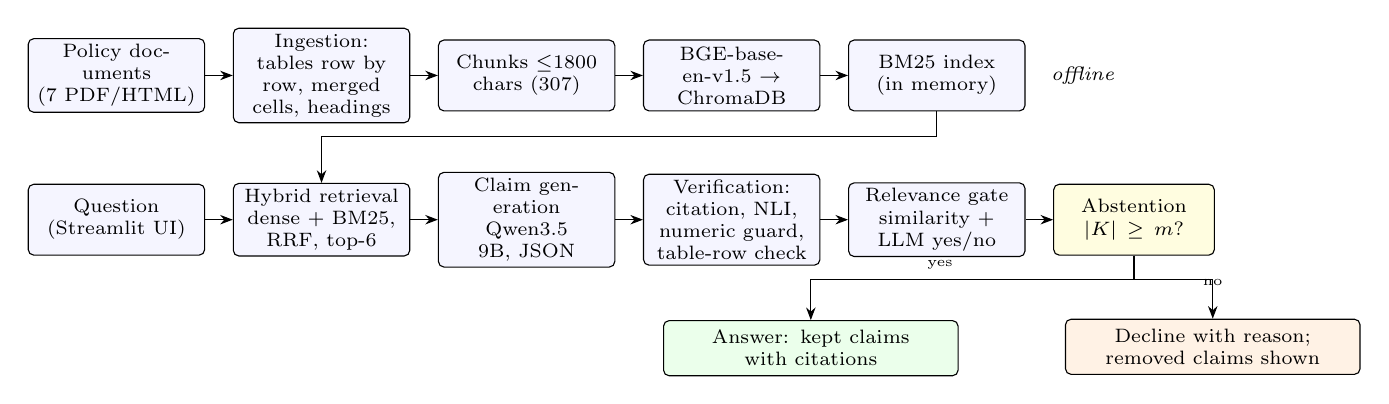
\begin{tikzpicture}[
  box/.style={draw, rounded corners=2pt, align=center, font=\scriptsize, minimum height=9mm, inner sep=2pt, text width=21mm, fill=blue!4},
  dec/.style={draw, rounded corners=2pt, align=center, font=\scriptsize, minimum height=9mm, inner sep=2pt, text width=19mm, fill=yellow!12},
  res/.style={draw, rounded corners=2pt, align=center, font=\scriptsize, minimum height=7mm, inner sep=2pt, text width=36mm},
  arr/.style={-{Stealth[length=1.6mm]}, thin},
  node distance=3mm and 3.5mm]
\node[box] (docs) {Policy documents\\(7 PDF/HTML)};
\node[box, right=of docs] (ing) {Ingestion: tables row by row, merged cells, headings};
\node[box, right=of ing] (chunks) {Chunks ${\le}1800$ chars (307)};
\node[box, right=of chunks] (dense) {BGE-base-en-v1.5 $\rightarrow$ ChromaDB};
\node[box, right=of dense] (bm25) {BM25 index\\(in memory)};
\node[font=\scriptsize\itshape, right=2mm of bm25] {offline};
\draw[arr] (docs)--(ing); \draw[arr] (ing)--(chunks); \draw[arr] (chunks)--(dense); \draw[arr] (dense)--(bm25);
\node[box, below=9mm of docs] (q) {Question\\(Streamlit UI)};
\node[box, right=of q] (ret) {Hybrid retrieval\\dense + BM25, RRF, top-6};
\node[box, right=of ret] (gen) {Claim generation\\Qwen3.5 9B, JSON};
\node[box, right=of gen] (ver) {Verification: citation, NLI, numeric guard, table-row check};
\node[box, right=of ver] (rel) {Relevance gate\\similarity + LLM yes/no};
\node[dec, right=of rel] (abs) {Abstention\\ $|K|\ge m$?};
\draw[arr] (q)--(ret); \draw[arr] (ret)--(gen); \draw[arr] (gen)--(ver); \draw[arr] (ver)--(rel); \draw[arr] (rel)--(abs);
\draw[arr] (bm25.south) -- ++(0,-3.2mm) -| (ret.north);
\node[res, fill=green!8, below=8mm of rel, xshift=-16mm] (ans) {Answer: kept claims with citations};
\node[res, fill=orange!10, below=8mm of abs, xshift=10mm] (decl) {Decline with reason; removed claims shown};
\draw[arr] (abs.south) -- ++(0,-3mm) -| node[pos=0.3, above, font=\tiny]{yes} (ans.north);
\draw[arr] (abs.south) -- ++(0,-3mm) -| node[pos=0.7, above, font=\tiny]{no} (decl.north);
\end{tikzpicture}
\caption{System architecture. The upper row is built once; the lower row runs per question. All components
run locally.}
\label{fig:arch}
\end{figure*}

% ---------------------------------------------------------------- Fig. 2
\begin{figure*}[t]
\centering
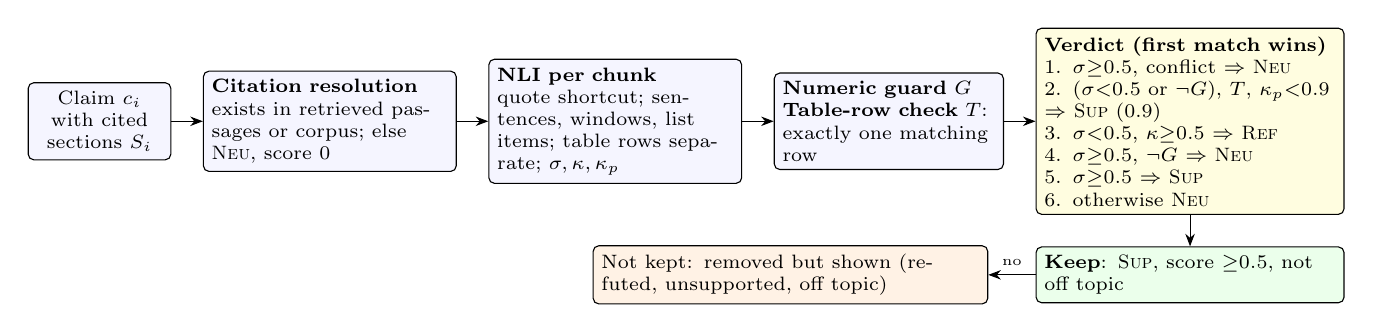
\begin{tikzpicture}[
  box/.style={draw, rounded corners=2pt, align=left, font=\scriptsize, inner sep=3pt, text width=30mm, fill=blue!4},
  arr/.style={-{Stealth[length=1.6mm]}, thin}, node distance=4mm]
\node[box, text width=16mm, align=center] (c) {Claim $c_i$ with cited sections $S_i$};
\node[box, right=of c] (cit) {\textbf{Citation resolution}\\exists in retrieved passages or corpus; else \NEU, score 0};
\node[box, right=of cit] (nli) {\textbf{NLI per chunk}\\quote shortcut; sentences, windows, list items; table rows separate; $\sigma,\kappa,\kappa_p$};
\node[box, right=of nli, text width=27mm] (tab) {\textbf{Numeric guard} $G$\\\textbf{Table-row check} $T$: exactly one matching row};
\node[box, right=of tab, text width=37mm, fill=yellow!12] (v) {\textbf{Verdict (first match wins)}\\1. $\sigma{\ge}0.5$, conflict $\Rightarrow$ \NEU\\2. ($\sigma{<}0.5$ or $\neg G$), $T$, $\kappa_p{<}0.9$ $\Rightarrow$ \SUP\ (0.9)\\3. $\sigma{<}0.5$, $\kappa{\ge}0.5$ $\Rightarrow$ \REF\\4. $\sigma{\ge}0.5$, $\neg G$ $\Rightarrow$ \NEU\\5. $\sigma{\ge}0.5$ $\Rightarrow$ \SUP\\6. otherwise \NEU};
\draw[arr] (c)--(cit); \draw[arr] (cit)--(nli); \draw[arr] (nli)--(tab); \draw[arr] (tab)--(v);
\node[box, below=4mm of v, text width=37mm, fill=green!8] (keep) {\textbf{Keep}: \SUP, score ${\ge}0.5$, not off topic};
\node[box, left=6mm of keep, text width=48mm, fill=orange!10] (rm) {Not kept: removed but shown (refuted, unsupported, off topic)};
\draw[arr] (v)--(keep); \draw[arr] (keep)--node[above, font=\tiny]{no}(rm);
\end{tikzpicture}
\caption{Path of one claim, following the implemented rules. Citation existence is checked separately from
semantic support. The numeric guard can veto but never grant support; the table-row check can grant but
never refute.}
\label{fig:claim}
\end{figure*}

% ===========================================================================
\section{Implementation and Experimental Setup}
% ===========================================================================
\subsection{Implementation}
The backend is Python 3.12 on Windows 11. The generator runs through Ollama on an RTX 4060 laptop GPU
(8~GB VRAM, 16~GB RAM); the encoder and verifier run on CPU (Table~\ref{tab:components}). 564 automated
tests run without any model, GPU or network. Repeated tuning runs at temperature 0 gave identical results;
an earlier configuration varied by about one question in 33.

\begin{table}[t]
\caption{Components and Runtime}
\label{tab:components}
\centering\scriptsize
\begin{tabular}{@{}lll@{}}
\toprule
Role & Component & Runs on\\
\midrule
Claims, relevance & Qwen3.5 9B (Ollama, Q4\_K\_M), no thinking & GPU\\
Embeddings & BAAI/bge-base-en-v1.5 (768-d) & CPU\\
NLI verifier & DeBERTa-v3-base-mnli-fever-anli & CPU, fp32\\
Table-row check, numeric guard & deterministic code & CPU\\
Vector / keyword index & ChromaDB / BM25 (in memory) & --\\
Interface & Streamlit & --\\
\bottomrule
\end{tabular}
\end{table}

\subsection{Corpus}
The corpus has seven official SRM Institute of Science and Technology (Kattankulathur) documents
(Table~\ref{tab:corpus}): 225 sections parsed, 222 indexed, 307 chunks. The scholarship web page (2023
onwards) and the amended Scholarship Categories PDF (2025--26) are both kept; they disagree on one figure
(Founder's Scholarship: IIT JEE rank ``top 20,000'' vs.\ ``up to 2000''), and each claim is verified against
its own source.

\begin{table}[t]
\caption{Policy Corpus}
\label{tab:corpus}
\centering\scriptsize
\begin{tabular}{@{}llrr@{}}
\toprule
Source & Fmt & Sect. & Chunks\\
\midrule
Academic Regulations 2021 & PDF & 63 & 78\\
Examination Policy & HTML & 61 & 90\\
Plagiarism Policy (2017) & PDF & 9 & 11\\
Scholarship Policy & HTML & 31 & 45\\
Scholarship Categories 2025--26 (Amended) & PDF & 13 & 22\\
Hostel Rules and Regulations (Jan 2025) & PDF & 35 & 38\\
Code of Conduct for Students & HTML & 13 & 23\\
\midrule
Total & & 225 & 307\\
\bottomrule
\end{tabular}
\end{table}

\subsection{Labelled sets and protocol}
Table~\ref{tab:sets} lists the labelled sets. Each question carries expected citation section(s) (any one
suffices), required values, known-wrong \emph{forbidden} values and a note. \textbf{All design decisions and
thresholds used the tuning split only.} The final test (99 questions) combines three sets written by people
other than the system's builder: 40 questions covering direct look-up, scenarios, multi-hop and
cross-document reasoning, calculations and version conflicts; 50 short, casual questions with table
look-ups, near misses and false premises; and 9 near-miss and false-premise questions written by a teammate
(five more were rejected because they repeated facts already tested). Before any run, every expected fact
was checked against the policy text; four answer-key sources were corrected, one unanswerable item was
marked a near miss, one question was relabelled answerable because the added PDF answers it, one answer was
updated for the added PDF, and two scoring rules were fixed: calculation questions earn
credit for the verified components, and three ambiguous items have an accepted answer. Questions were given
to the system without their type tags. The test was run \emph{once} on the frozen system.

\begin{table}[t]
\caption{Labelled Sets and Final-Test Categories}
\label{tab:sets}
\centering\scriptsize
\begin{tabular}{@{}lrll@{}}
\toprule
Set & Size & Use & Written by\\
\midrule
Adversarial questions & 64 & 33 tuning / 31 held-out (v1) & author\\
Fresh check set & 49 & development check & author\\
Independent questions & 40 & held-out (v1) & teammate\\
Labelled claims & 85 & 44 tuning / 41 held-out (v1) & author\\
\textbf{Final test} & \textbf{99} & \textbf{held-out (v2), run once} & \textbf{independent}\\
\midrule
\multicolumn{4}{@{}l}{Final test by category: numeric/table/calculation 34, unanswerable 16,}\\
\multicolumn{4}{@{}l}{false premise 14, negation/exception 17, cross-policy/document 18;}\\
\multicolumn{4}{@{}l}{83 answerable / 16 unanswerable.}\\
\bottomrule
\end{tabular}
\end{table}

\subsection{Scoring and metrics}
Each question ends in one outcome: correct; correct abstention (declined, unanswerable); false abstention
(declined, answerable); answered-unanswerable; wrong value (a kept claim contains a forbidden value); wrong
citation (no kept claim cites an expected section); incomplete (a required value missing). With $N$
questions,
\begin{equation}
\mathrm{Acc}=\frac{N_{\mathrm{c}}+N_{\mathrm{ca}}}{N},\qquad
\mathrm{Hall}=\frac{N_{\mathrm{wv}}+N_{\mathrm{au}}}{N},
\end{equation}
where $N_{\mathrm{c}}$, $N_{\mathrm{ca}}$, $N_{\mathrm{wv}}$ and $N_{\mathrm{au}}$ count correct, correct
abstention, wrong value and answered-unanswerable outcomes.
\emph{Wrong when answering} is answers with any error over answers given; \emph{citation accuracy} is
answered questions with a kept claim on an expected section over answered questions. Intervals are 95\%
Wilson intervals \cite{wilson1927}:
\begin{equation}
\frac{\hat p+\frac{z^2}{2n}\pm z\sqrt{\frac{\hat p(1-\hat p)}{n}+\frac{z^2}{4n^2}}}{1+\frac{z^2}{n}},\quad z=1.96.
\end{equation}
For $k=0$ the upper limit is $z^2/(n+z^2)$, e.g.\ $3.84/102.84=3.7\%$ for $n=99$: a score of 0\% means that
no failure was observed, not that none is possible. The \emph{verification-off} condition re-scores the same
generated claims as if all had been kept.

\subsection{Disclosures}\label{sec:disclosure}
(i) After the version-1 held-out run, two labels found wrong on inspection were corrected and the saved
outputs rescored without rerunning the model \cite{prev}. (ii) The audit showed that held-out item
\code{num-011} (attendance code at 90\%) had been labelled from damaged text; its label now expects code
``9''; the version-1 numbers do not change because that question was declined. (iii) After re-ingestion, 29
expected citations were remapped to renamed sections, each checked by hand. (iv) Text before a document's
first detected heading is not indexed, so plagiarism type~1 is missing; this was found while converting the
final test and deliberately not repaired, so item \code{fb-29} measures it. (v) Later changes proposed by
a teammate (a cross-encoder relevance judge, re-ranking and others) were not part of the tested system.

% ===========================================================================
\section{Results and Discussion}
% ===========================================================================
\subsection{Development on the tuning split}
Table~\ref{tab:dev} traces the tuning split (33 questions) through the changes. A teammate proposed four
retrieval add-ons (LLM-written section summaries attached to every chunk, an entity-overlap boost, an
audience filter and 800-character chunks). Switching them off one at a time on the tuning split showed the
summaries to be the main cost: removing them recovered 6--12 points, because every chunk of a section
carried the same summary and the exact rule (for example the 50\% pass mark) dropped out of the top six.
All four were switched off and the 1800-character chunks restored. After the ingestion repair the verifier
reached precision 100\% (24/24, CI 86.2--100) and a false-accept rate of 0\% (0/20, CI 0--16.1) on the
tuning claims, against 96\% and 5\% before. The table-row check left tuning unchanged and raised the fresh
check set from 83.7\% to 85.7\%. Moving from Qwen3 4B to Qwen3.5 9B removed the remaining tuning
hallucination but declined more answerable questions; a prompt rule for false premises recovered three of
them.

\begin{table}[t]
\caption{Development on the Tuning Split (33 Questions)}
\label{tab:dev}
\centering\scriptsize
\begin{tabular}{@{}llrrr@{}}
\toprule
Stage & Model & Acc. & Hall. & False abst.\\
\midrule
Audit (before improvements) & 4B & 57.6\% & 18.2\% & 4/26\\
Version 1 (frozen) & 4B & 78.8\% & 3.0\% & 2/26\\
+ retrieval add-ons (all on) & 4B & 69.7\% & 6.1--9.1\% & 4--5/26\\
\quad add-ons off, 1800-char chunks & 4B & 81.8\% & 3.0\% & 3/26\\
Repaired ingestion + table-row check & 4B & 75.8\% & 3.0\% & 4/26\\
Qwen3.5 9B & 9B & 72.7\% & 0.0\% & 9/26\\
+ false-premise rule (\textbf{final}) & 9B & \textbf{75.8\%} & \textbf{0.0\%} & 6/26\\
\bottomrule
\multicolumn{5}{@{}l}{\scriptsize Final row: 25/33, CI 59.0--87.2; hallucination 0/33, CI 0--10.4.}
\end{tabular}
\end{table}

\subsection{Final test: end-to-end results}
Table~\ref{tab:final} gives the headline results, and Fig.~\ref{fig:onoff} the comparison with
verification switched off. The system declined 15 of 16 unanswerable questions. The automatic scorer counted
three hallucinations (3.0\%); read by hand, none states a false fact. In two (score-table questions) the
system listed every row of the table, all verified and true, including the correct one, and the scorer
flagged the other rows' percentages; in the third the system answered that the policy ``does not specify a
number of days; the receipt must be submitted while checking in'', the correct near-miss answer, which the
scorer counts as answering an unanswerable question. Without verification the same claims give 9.1\%
automatic hallucination.

\begin{table}[t]
\caption{Final Test (99 Questions, Run Once): Verification On vs.\ Off}
\label{tab:final}
\centering\scriptsize
\begin{tabular}{@{}lll@{}}
\toprule
Metric & On & Off\\
\midrule
Accuracy & 62.6\% [52.8--71.5] (62/99) & 79.8\% [70.8--86.5]\\
Hallucination (automatic) & 3.0\% [1.0--8.5] (3/99) & 9.1\% [4.9--16.4]\\
Hallucination (by hand) & 0\% [0.0--3.7] (0/99) & --\\
Correct abstention & 93.8\% [71.7--98.9] (15/16) & 75.0\%\\
False abstention & 30.1\% [21.3--40.7] (25/83) & 3.6\%\\
Wrong when answering & 20.3\% [12.0--32.3] (12/59) & --\\
Citation accuracy & 98.3\% & 97.5\%\\
Claims generated / kept / removed & 271 / 138 / 133 & --\\
Median latency per question & 11.4 s (p95 30.0 s) & --\\
\bottomrule
\end{tabular}
\end{table}

\begin{figure}[t]
\centering
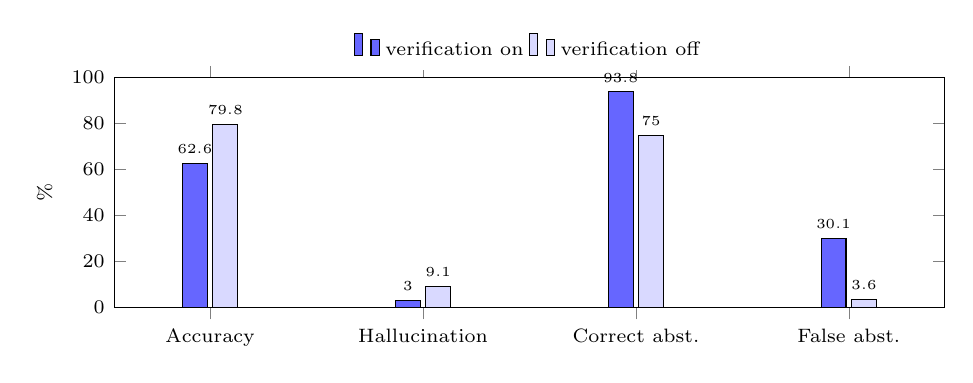
\begin{tikzpicture}
\begin{axis}[ybar, bar width=9pt, width=\columnwidth, height=45mm, ymin=0, ymax=100,
  symbolic x coords={A,H,C,F}, xtick=data, xticklabels={Accuracy,Hallucination,Correct abst.,False abst.},
  ticklabel style={font=\scriptsize}, ylabel={\%}, ylabel style={font=\scriptsize},
  nodes near coords, nodes near coords style={font=\tiny},
  legend style={font=\scriptsize, at={(0.5,1.03)}, anchor=south, legend columns=2, draw=none},
  enlarge x limits=0.15]
\addplot[fill=blue!60] coordinates {(A,62.6) (H,3.0) (C,93.8) (F,30.1)};
\addplot[fill=blue!15] coordinates {(A,79.8) (H,9.1) (C,75.0) (F,3.6)};
\legend{verification on, verification off}
\end{axis}
\end{tikzpicture}
\caption{Final test, verification on vs.\ off (same generated claims). Hallucination is the automatic
count; read by hand, the ``on'' condition has none.}
\label{fig:onoff}
\end{figure}

\subsection{Outcomes and confusion matrix}
Table~\ref{tab:outcomes} gives the outcome counts. As in version~1, the dominant error is a wrongly
withheld answer (25), not a wrong one (12 answers with any error, of which the 8 ``incomplete'' answers
include values written differently, e.g.\ ``1 year'' for ``one year'').

\begin{table}[t]
\caption{Final Test: Outcomes and Answer/Abstain Matrix}
\label{tab:outcomes}
\centering\scriptsize
\begin{tabular}{@{}lr@{\hspace{8mm}}lrr@{}}
\toprule
Outcome & No. & & Answered & Declined\\
\midrule
Correct & 47 & Answerable (83) & 58 & 25\\
Correct abstention & 15 & Unanswerable (16) & 1 & 15\\
False abstention & 25 & & & \\
Incomplete & 8 & & & \\
Wrong value & 2 & & & \\
Answered unanswerable & 1 & & & \\
Wrong citation & 1 & & & \\
\midrule
Total & 99 & & 59 & 40\\
\bottomrule
\end{tabular}
\end{table}

\subsection{Accuracy by category and by source}
Unanswerable (15/16) and negation/exception (13/17, 76.5\%) questions are handled best; cross-policy
reaches 12/18 (66.7\%) and false premise 8/14 (57.1\%); numeric, table and calculation questions are weakest
at 14/34 (41.2\%) (Table~\ref{tab:cat}). By source, the 40 reasoning-heavy questions scored 20/40 (50.0\%),
the 50 short questions 34/50 (68.0\%) and the 9 near-miss and false-premise questions 8/9. Categories hold
14--34 items, so single percentages are fragile.

\begin{table}[t]
\caption{Final Test: Accuracy by Category}
\label{tab:cat}
\centering\scriptsize
\begin{tabular}{@{}lll@{}}
\toprule
Category & Correct & 95\% CI\\
\midrule
Unanswerable & 15/16 (93.8\%) & 71.7--98.9\\
Negation/exception & 13/17 (76.5\%) & 52.7--90.4\\
Cross-policy/document & 12/18 (66.7\%) & 43.7--83.7\\
False premise & 8/14 (57.1\%) & 32.6--78.6\\
Numeric/table/calculation & 14/34 (41.2\%) & 26.4--57.8\\
\bottomrule
\end{tabular}
\end{table}

\subsection{Where the false abstentions come from}
Of the 25 declined answerable questions, 17 had claims that were verified as true and then rejected by the
relevance gate (all 34 removed true claims in those questions), 5 had claims that could not be verified, and
in 3 the model produced no claim. The gate's yes/no prompt and thresholds were tuned with Qwen3 4B; Qwen3.5
9B answers it far more strictly. This explains most of the 17-point gap to the verification-off condition:
with the stronger generator, the raw answers are already better, and the checks discard about a fifth of
the correct ones. The gate was not changed after the final run, since that would amount to tuning on the
test.

\subsection{The table-row check in use}
Fig.~\ref{fig:screen} shows the check on ``What attendance code is given to a student with 90\% attendance?''.
The NLI model cannot place 90\% in ``85 to 94\%''; the check finds the single matching row and supports
``Code~9'', while a second claim that restates the band is removed by the numeric guard because ``85\%'' is
not written in the row. During development each rule of the check was added because an earlier version
supported a deliberately wrong claim (a different scheme named, a figure under the wrong fee column, or a
value from an adjacent label in the same cell); 29 unit tests keep these cases. On the final test it granted
support once, correctly.

\begin{figure}[t]
\centering
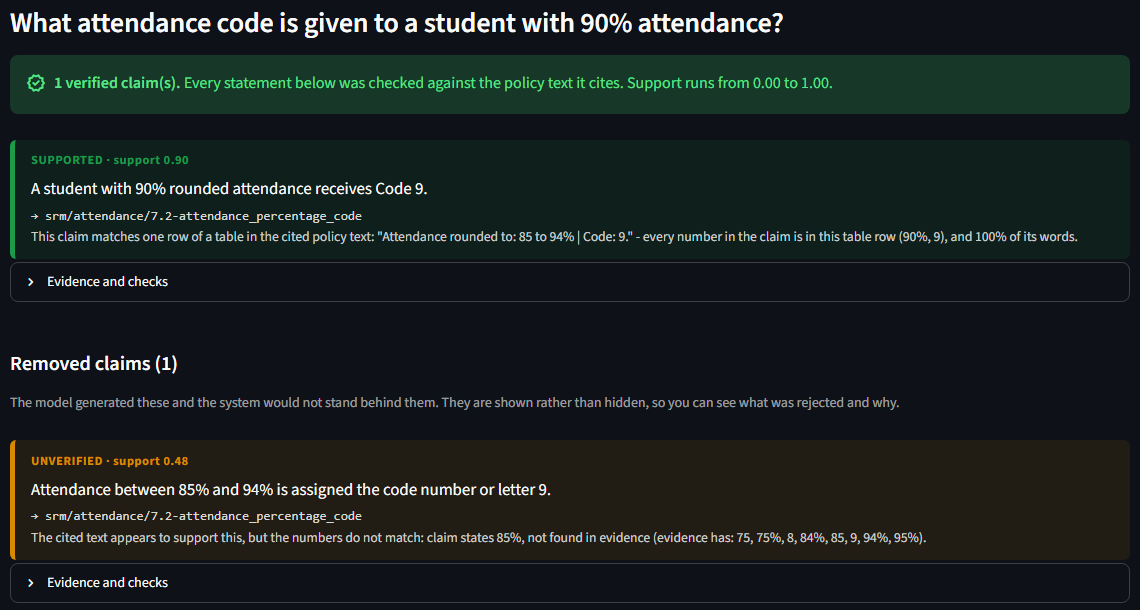
\includegraphics[width=\columnwidth]{fig_table_row_check.png}
\caption{The interface on a table look-up: the claim ``Code~9'' is supported by the table-row check
(score 0.90); a second claim is removed by the numeric guard and shown with the reason.}
\label{fig:screen}
\end{figure}

\subsection{Comparison with version 1}
Version 1 (Qwen3 4B, six documents) was evaluated earlier on different held-out questions
\cite{prev}: 77.5\% [62.5--87.7] accuracy and 0/40 hallucination on 40 independent questions, 74.2\% and
1/31 on 31 held-out adversarial questions, and a verifier precision of 88.5\% with 3 of 18 unsupported claims
accepted, all ``right number, wrong row''. The final test of version 2 is harder: 26 of its 99 questions are
scenarios, multi-hop questions, version conflicts or calculations. Because the model, corpus and questions
all differ, the two versions should each be compared only with their own verification-off condition. In both,
verification removed the observed false statements; with the 4B generator it also raised accuracy slightly,
whereas with the 9B generator it lowered accuracy because of the relevance gate.

\subsection{Latency}
The median question takes 11.4~s (p95 30.0~s): generation 6.2~s and verification with the relevance gate
4.0~s at the median; retrieval is under 0.1~s.

\subsection{Error analysis}
Table~\ref{tab:errors} lists the observed failure types. Besides the relevance gate, three are visible in
individual answers. A correction that repeats the question's wrong figure (``a maximum of 10\%, not 25\%'')
is vetoed by the numeric guard because the repeated figure is not in the evidence. A version conflict between
the two scholarship documents is not surfaced: the claim citing both is supported by the page and kept,
without showing that the PDF gives a different figure. And when the model capitalises header words
(``Tuition Fee Waiver''), the table-row check's name rule can reject a correct row.

\begin{table}[t]
\caption{Error Analysis (Final Test)}
\label{tab:errors}
\centering\scriptsize
\begin{tabular}{@{}p{30mm}p{20mm}p{25mm}@{}}
\toprule
Failure & Evidence & Likely source\\
\midrule
True claims rejected as off topic & 17 of 25 false abstentions & gate tuned for 4B model\\
Table answers not verified & numeric/table 14/34 & NLI on rows; name rule\\
Correction with the question's figure vetoed & false-premise items & chunk-level numeric guard\\
Version conflict not surfaced & IIT JEE cut-off item & conflict rule needs a contradiction\\
Whole table listed & 2 score-table items & generator verbosity\\
Unindexed text before first heading & \code{fb-29} & ingestion\\
Computed totals & 1/4 calculation items & verify-only design\\
\bottomrule
\end{tabular}
\end{table}

\subsection{Limitations and threats to validity}
\textit{Scale and scope.} 99 questions give intervals of about $\pm$10 points; one institution and seven
documents, so transfer is untested. \textit{Scoring.} The automatic scorer is a first pass: its three
``hallucinations'' were artefacts, and multi-part, calculation and near-miss answers need grading by hand
against the rubric. \textit{Tuning mismatch.} Prompts and relevance thresholds were tuned with the 4B model
and not re-tuned for the 9B model before the final test. \textit{Builder involvement.} The questions and
answers were written by others, but the builder converted them to the scoring format. \textit{Label
changes} are disclosed in Section~\ref{sec:disclosure}. \textit{Missing comparisons.} There is no external
fact-checking baseline and no larger generator; the development changes were made in sequence, and only the
retrieval add-ons were ablated one at a time, on the tuning split. \textit{Definition.} Hallucination counts
forbidden values and answered-unanswerable outcomes; it is a lower bound, which is why every flagged case
was read by hand.

% ===========================================================================
\section{Conclusion and Future Work}
% ===========================================================================
We presented a local policy question-answering assistant that verifies atomic claims against cited
sections, reads table rows without losing their structure, resolves range look-ups with a deterministic
check, and declines when no verified, relevant claim remains. On 99 independently written questions run
once, it declined 15 of 16 unanswerable questions and, read by hand, presented no false statement as
verified, while the same answers without verification contained flagged errors in about one question in
eleven. The cost is visible: 30\% of answerable questions were declined, mostly by a relevance gate tuned
for a smaller model, so accuracy was 62.6\% against 79.8\% with verification off. An audit also showed that
an ingestion heuristic can silently delete table values and corrupt evaluation labels, so the stored text
must be checked against the source documents.

Future work follows from the error analysis: re-tune the relevance gate for the current generator on the
tuning split, which addresses up to 17 of the 25 false abstentions; let the numeric guard ignore figures
taken from the question; surface version conflicts between documents; broaden the table-row check; index
text before the first heading; compare with a dedicated fact-checker \cite{tang2024minicheck} and larger
generators; and extend to larger independently written sets \cite{ribeiro2020checklist} and more
institutions.

\section*{Acknowledgment}
The authors thank their guide, Dr. P. Akilandeswari, and the teammates and contributors who independently
wrote the evaluation question sets and answer keys.

% ===========================================================================
\begin{thebibliography}{00}
\bibitem{lewis2020rag} P. Lewis \emph{et al.}, ``Retrieval-augmented generation for knowledge-intensive NLP tasks,'' in \emph{Adv. Neural Inf. Process. Syst.}, vol. 33, 2020, pp. 9459--9474.
\bibitem{maynez2020faithfulness} J. Maynez, S. Narayan, B. Bohnet, and R. McDonald, ``On faithfulness and factuality in abstractive summarization,'' in \emph{Proc. 58th Annu. Meeting Assoc. Comput. Linguistics (ACL)}, 2020, pp. 1906--1919.
\bibitem{huang2024selfcorrect} J. Huang \emph{et al.}, ``Large language models cannot self-correct reasoning yet,'' in \emph{Proc. Int. Conf. Learn. Representations (ICLR)}, 2024.
\bibitem{koreeda2021contractnli} Y. Koreeda and C. D. Manning, ``ContractNLI: A dataset for document-level natural language inference for contracts,'' in \emph{Findings Assoc. Comput. Linguistics: EMNLP 2021}, 2021, pp. 1907--1919.
\bibitem{ravichander2019equate} A. Ravichander, A. Naik, C. Rose, and E. Hovy, ``EQUATE: A benchmark evaluation framework for quantitative reasoning in natural language inference,'' in \emph{Proc. 23rd Conf. Comput. Natural Lang. Learn. (CoNLL)}, 2019, pp. 349--361.
\bibitem{kamath2020selective} A. Kamath, R. Jia, and P. Liang, ``Selective question answering under domain shift,'' in \emph{Proc. 58th Annu. Meeting Assoc. Comput. Linguistics (ACL)}, 2020, pp. 5684--5696.
\bibitem{ribeiro2020checklist} M. T. Ribeiro, T. Wu, C. Guestrin, and S. Singh, ``Beyond accuracy: Behavioral testing of NLP models with CheckList,'' in \emph{Proc. 58th Annu. Meeting Assoc. Comput. Linguistics (ACL)}, 2020, pp. 4902--4912.
\bibitem{robertson2009bm25} S. Robertson and H. Zaragoza, ``The probabilistic relevance framework: BM25 and beyond,'' \emph{Found. Trends Inf. Retr.}, vol. 3, no. 4, pp. 333--389, 2009.
\bibitem{cormack2009rrf} G. V. Cormack, C. L. A. Clarke, and S. Buettcher, ``Reciprocal rank fusion outperforms Condorcet and individual rank learning methods,'' in \emph{Proc. 32nd Int. ACM SIGIR Conf. Res. Develop. Inf. Retr.}, 2009, pp. 758--759.
\bibitem{xiao2023cpack} S. Xiao, Z. Liu, P. Zhang, N. Muennighoff, D. Lian, and J.-Y. Nie, ``C-Pack: Packed resources for general Chinese embeddings,'' arXiv:2309.07597, 2023.
\bibitem{bge} Beijing Academy of Artificial Intelligence (BAAI), ``BAAI/bge-base-en-v1.5,'' Hugging Face model card. [Online]. Available: \url{https://huggingface.co/BAAI/bge-base-en-v1.5}. Accessed: Nov. 20, 2026.
\bibitem{laban2022summac} P. Laban, T. Schnabel, P. N. Bennett, and M. A. Hearst, ``SummaC: Re-visiting NLI-based models for inconsistency detection in summarization,'' \emph{Trans. Assoc. Comput. Linguistics}, vol. 10, pp. 163--177, 2022.
\bibitem{he2021debertav3} P. He, J. Gao, and W. Chen, ``DeBERTaV3: Improving DeBERTa using ELECTRA-style pre-training with gradient-disentangled embedding sharing,'' arXiv:2111.09543, 2021.
\bibitem{laurer} M. Laurer, ``DeBERTa-v3-base-mnli-fever-anli,'' Hugging Face model card. [Online]. Available: \url{https://huggingface.co/MoritzLaurer/DeBERTa-v3-base-mnli-fever-anli}. Accessed: Nov. 19, 2026.
\bibitem{guo2017calibration} C. Guo, G. Pleiss, Y. Sun, and K. Q. Weinberger, ``On calibration of modern neural networks,'' in \emph{Proc. 34th Int. Conf. Mach. Learn. (ICML)}, PMLR vol. 70, 2017, pp. 1321--1330.
\bibitem{tang2024minicheck} L. Tang, P. Laban, and G. Durrett, ``MiniCheck: Efficient fact-checking of LLMs on grounding documents,'' arXiv:2404.10774, 2024.
\bibitem{qwen3} A. Yang \emph{et al.}, ``Qwen3 technical report,'' arXiv:2505.09388, 2025.
\bibitem{qwen35} Qwen Team, ``qwen3.5,'' Ollama model library. [Online]. Available: \url{https://ollama.com/library/qwen3.5}. Accessed: Nov. 20, 2026.
\bibitem{pymupdf} Artifex Software, ``PyMuPDF documentation.'' [Online]. Available: \url{https://pymupdf.readthedocs.io}. Accessed: Nov. 20, 2026.
\bibitem{wilson1927} E. B. Wilson, ``Probable inference, the law of succession, and statistical inference,'' \emph{J. Amer. Statist. Assoc.}, vol. 22, no. 158, pp. 209--212, 1927.
\bibitem{prev} D. Nambiar, A. Verma, and T. Suman, ``Hallucination and citation verifier for policy question answering (version 1),'' project report, Dept. Comput. Technol., SRM Inst. Sci. Technol., Nov. 2026.
\end{thebibliography}

\end{document}
